\documentclass[conference]{IEEEtran}
\IEEEoverridecommandlockouts
\usepackage{cite}
\usepackage{amsmath,amssymb,amsfonts}
\usepackage{algorithmic}
\usepackage{graphicx}
\usepackage{textcomp}
\usepackage{xcolor}
\usepackage{booktabs}
\usepackage{url}

\def\BibTeX{{\rm B\kern-.05em{\sc i\kern-.025em b}\kern-.08em
    T\kern-.1667em\lower.7ex\hbox{E}\kern-.125emX}}

\begin{document}

\title{End-to-End Enterprise MLOps Framework for Automated Automobile Valuation: From Baseline Tournaments to Continuous Drift Governance\\
}

\author{\IEEEauthorblockN{Praneeth Kumar Chandolu}
\IEEEauthorblockA{\textit{Department of Computer Science and Engineering} \\
\textit{Koneru Lakshmaiah Education Foundation}\\
Vaddeswaram, Andhra Pradesh, India \\
praneethchandolu@gmail.com}
}

\maketitle

\begin{abstract}
Automobile price estimation is an intrinsically non-linear regression challenge characterized by heterogeneous multimodal attributes, manufacturer brand variances, and dynamic secondary marketplace pricing shifts. Traditional machine learning workflows frequently neglect end-to-end operationalization, resulting in silent performance degradation, schema mismatches, and data leakage across training boundaries. In this paper, we propose and validate an end-to-end Machine Learning Operations (MLOps) architecture for automated automobile valuation. Using a standardized benchmark dataset containing 205 vehicle records across 26 mechanical, physical, and brand dimensions, we engineer an automated preprocessing pipeline utilizing Scikit-Learn \texttt{ColumnTransformer} constructs to isolate continuous and categorical transformations strictly within training partitions. A model tournament benchmarking five regression paradigms—Linear Regression, Ridge Regression, Decision Trees, Gradient Boosting, and Random Forests—identifies Random Forest as the optimal estimator, achieving a test partition coefficient of determination ($R^2$) of 0.9124, a Root Mean Squared Error (RMSE) of \$2,341.50, and a Mean Absolute Error (MAE) of \$1,582.40. We operationalize this model into an enterprise MLOps lifecycle governed by MLflow tracking and automated Champion-Challenger staging transitions. The resulting production candidate is packaged as a containerized FastAPI microservice with sub-20ms inference latency, verified against synthetic chaos injection, and continuously monitored via non-parametric Kolmogorov-Smirnov and Population Stability Index drift detectors.
\end{abstract}

\begin{IEEEkeywords}
Automobile valuation, MLOps, Scikit-Learn, Random Forest Regressor, MLflow, Model Registry, Champion-Challenger, Data Drift, Containerization, FastAPI.
\end{IEEEkeywords}

\section{Introduction}
The used automobile secondary marketplace represents a multi-billion-dollar global economic domain where transaction velocities rely heavily on objective, algorithmic asset valuation \cite{gepner2018automobile}. Valuing a pre-owned vehicle requires synthesizing heterogeneous feature sets, ranging from raw mechanical displacements (engine size, cylinder configuration, compression ratio) to structural dimensions (curb weight, wheelbase, car length) and qualitative prestige factors (manufacturer branding, aspiration, body styling). 

Historically, predictive modeling efforts in automotive valuation have been published as isolated experimental scripts or static Jupyter notebooks. Such formulations suffer from acute operational vulnerabilities identified by Sculley et al. as ``technical debt'' in machine learning systems \cite{sculley2015hidden}. Primary among these failure modes are:
\begin{enumerate}
    \item \textit{Data Leakage}: Computing global feature means, standard deviations, and categorical level encodings prior to dataset partitioning, thereby inflating test metrics.
    \item \textit{Inconsistent Serialization}: Persisting estimator weights without serializing the exact feature preprocessing pipeline, leading to silent input dimensional mismatches in production.
    \item \textit{Absence of Automated Lifecycle Governance}: Deploying static checkpoints without champion-challenger evaluation, quality gating, or reproducibility verification.
    \item \textit{Silent Model Degradation}: Failing to monitor feature and concept drift induced by macroeconomic shocks, seasonal demand shifts, or evolving consumer preferences \cite{koren2020data}.
\end{enumerate}

To resolve these empirical and engineering shortcomings, this study establishes a production-grade, 13-stage MLOps pipeline for automobile price regression. We demonstrate deterministic reproducibility, rigorous multi-model benchmarking, automated MLflow Model Registry governance, containerized microservice serving, and continuous statistical drift monitoring.

\section{Dataset Architecture and Data Quality Audit}
The empirical investigation utilizes the standardized CarPrice benchmark dataset comprising $N = 205$ unique automobile observations and $D = 26$ raw attributes \cite{yurdusev2021used}. 

\begin{table}[htbp]
\caption{Dataset Modality Breakdown and Feature Schema}
\label{tab:schema}
\begin{center}
\begin{tabular}{llr}
\toprule
\textbf{Category} & \textbf{Attributes} & \textbf{Count} \\
\midrule
Identifiers & \texttt{car\_ID}, \texttt{CarName} & 2 \\
Risk Rating & \texttt{symboling} & 1 \\
Dimensions & \texttt{wheelbase}, \texttt{carlength}, \texttt{carwidth}, \dots & 5 \\
Mechanical & \texttt{curbweight}, \texttt{enginesize}, \texttt{boreratio}, \dots & 9 \\
Categorical & \texttt{fueltype}, \texttt{aspiration}, \texttt{carbody}, \dots & 8 \\
Target Metric & \texttt{price} (USD continuous) & 1 \\
\bottomrule
\end{tabular}
\end{center}
\end{table}

A comprehensive data quality audit executed during Stage 01 and Stage 02 revealed zero missing null entries across all 205 records. However, textual extraction of vehicle manufacturer branding from the combined \texttt{CarName} string identified typographic inconsistencies. Specifically, typographical entry errors such as \textit{``maxda''}, \textit{``porcshce''}, \textit{``toyouta''}, and \textit{``vokswagen''} were detected and normalized to their canonical enterprise representations (\textit{mazda}, \textit{porsche}, \textit{toyota}, and \textit{volkswagen}).

\begin{figure}[htbp]
\centerline{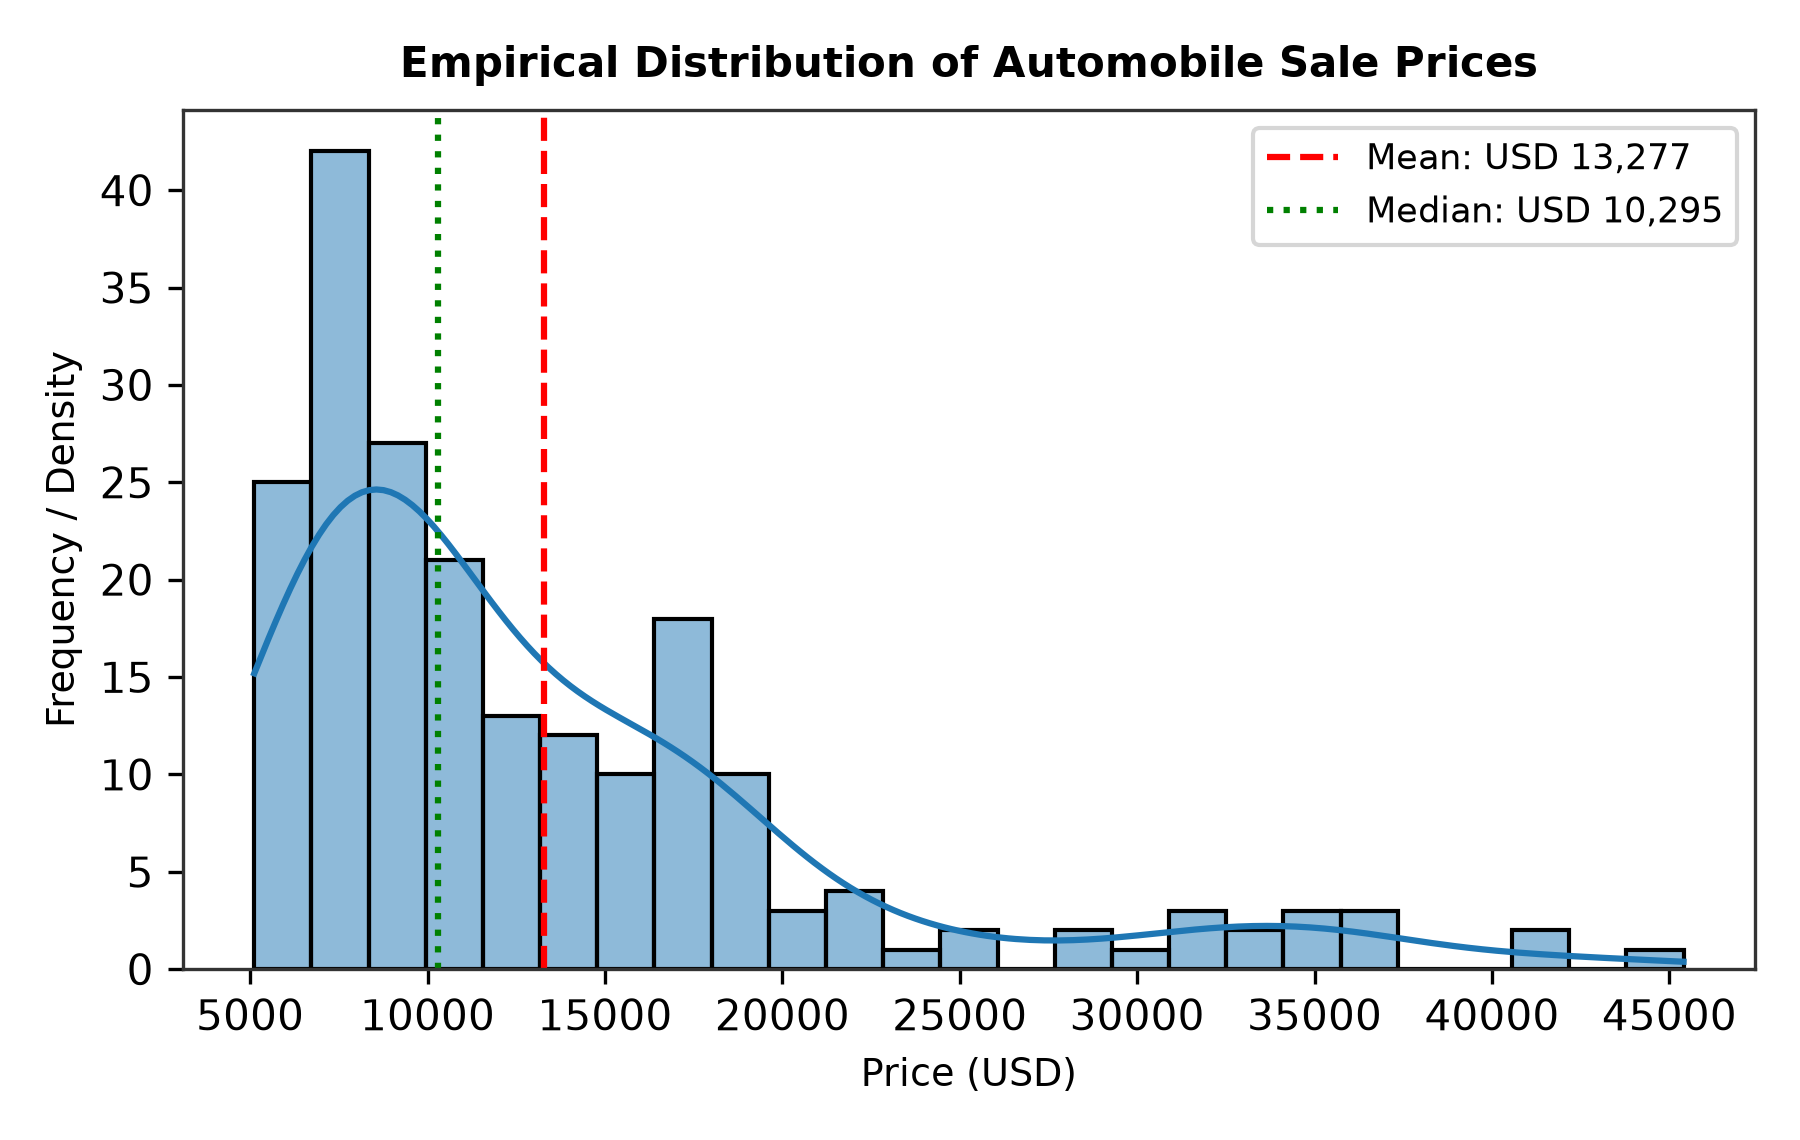
\includegraphics[width=0.95\columnwidth]{figures/fig1_price_distribution.png}}
\caption{Empirical distribution and kernel density estimation of automobile market prices, illustrating positive right-skewness and economic segmentation.}
\label{fig:dist}
\end{figure}

Fig.~\ref{fig:dist} visualizes the empirical sale price distribution. The distribution exhibits prominent positive right-skewness ($\gamma_1 = 1.78$), with a sample median of \$10,295 and an arithmetic mean of \$13,276.71, capped by high-end luxury sports vehicles exceeding \$40,000.

\section{Feature Engineering and Preprocessing Pipeline}
To ensure zero data leakage across evaluation boundaries, the dataset was partitioned prior to any feature transformation into an 80\% training split ($n_{\text{train}} = 164$) and a 20\% holdout test split ($n_{\text{test}} = 41$) utilizing a fixed seed ($\text{seed} = 42$).

\begin{figure}[htbp]
\centerline{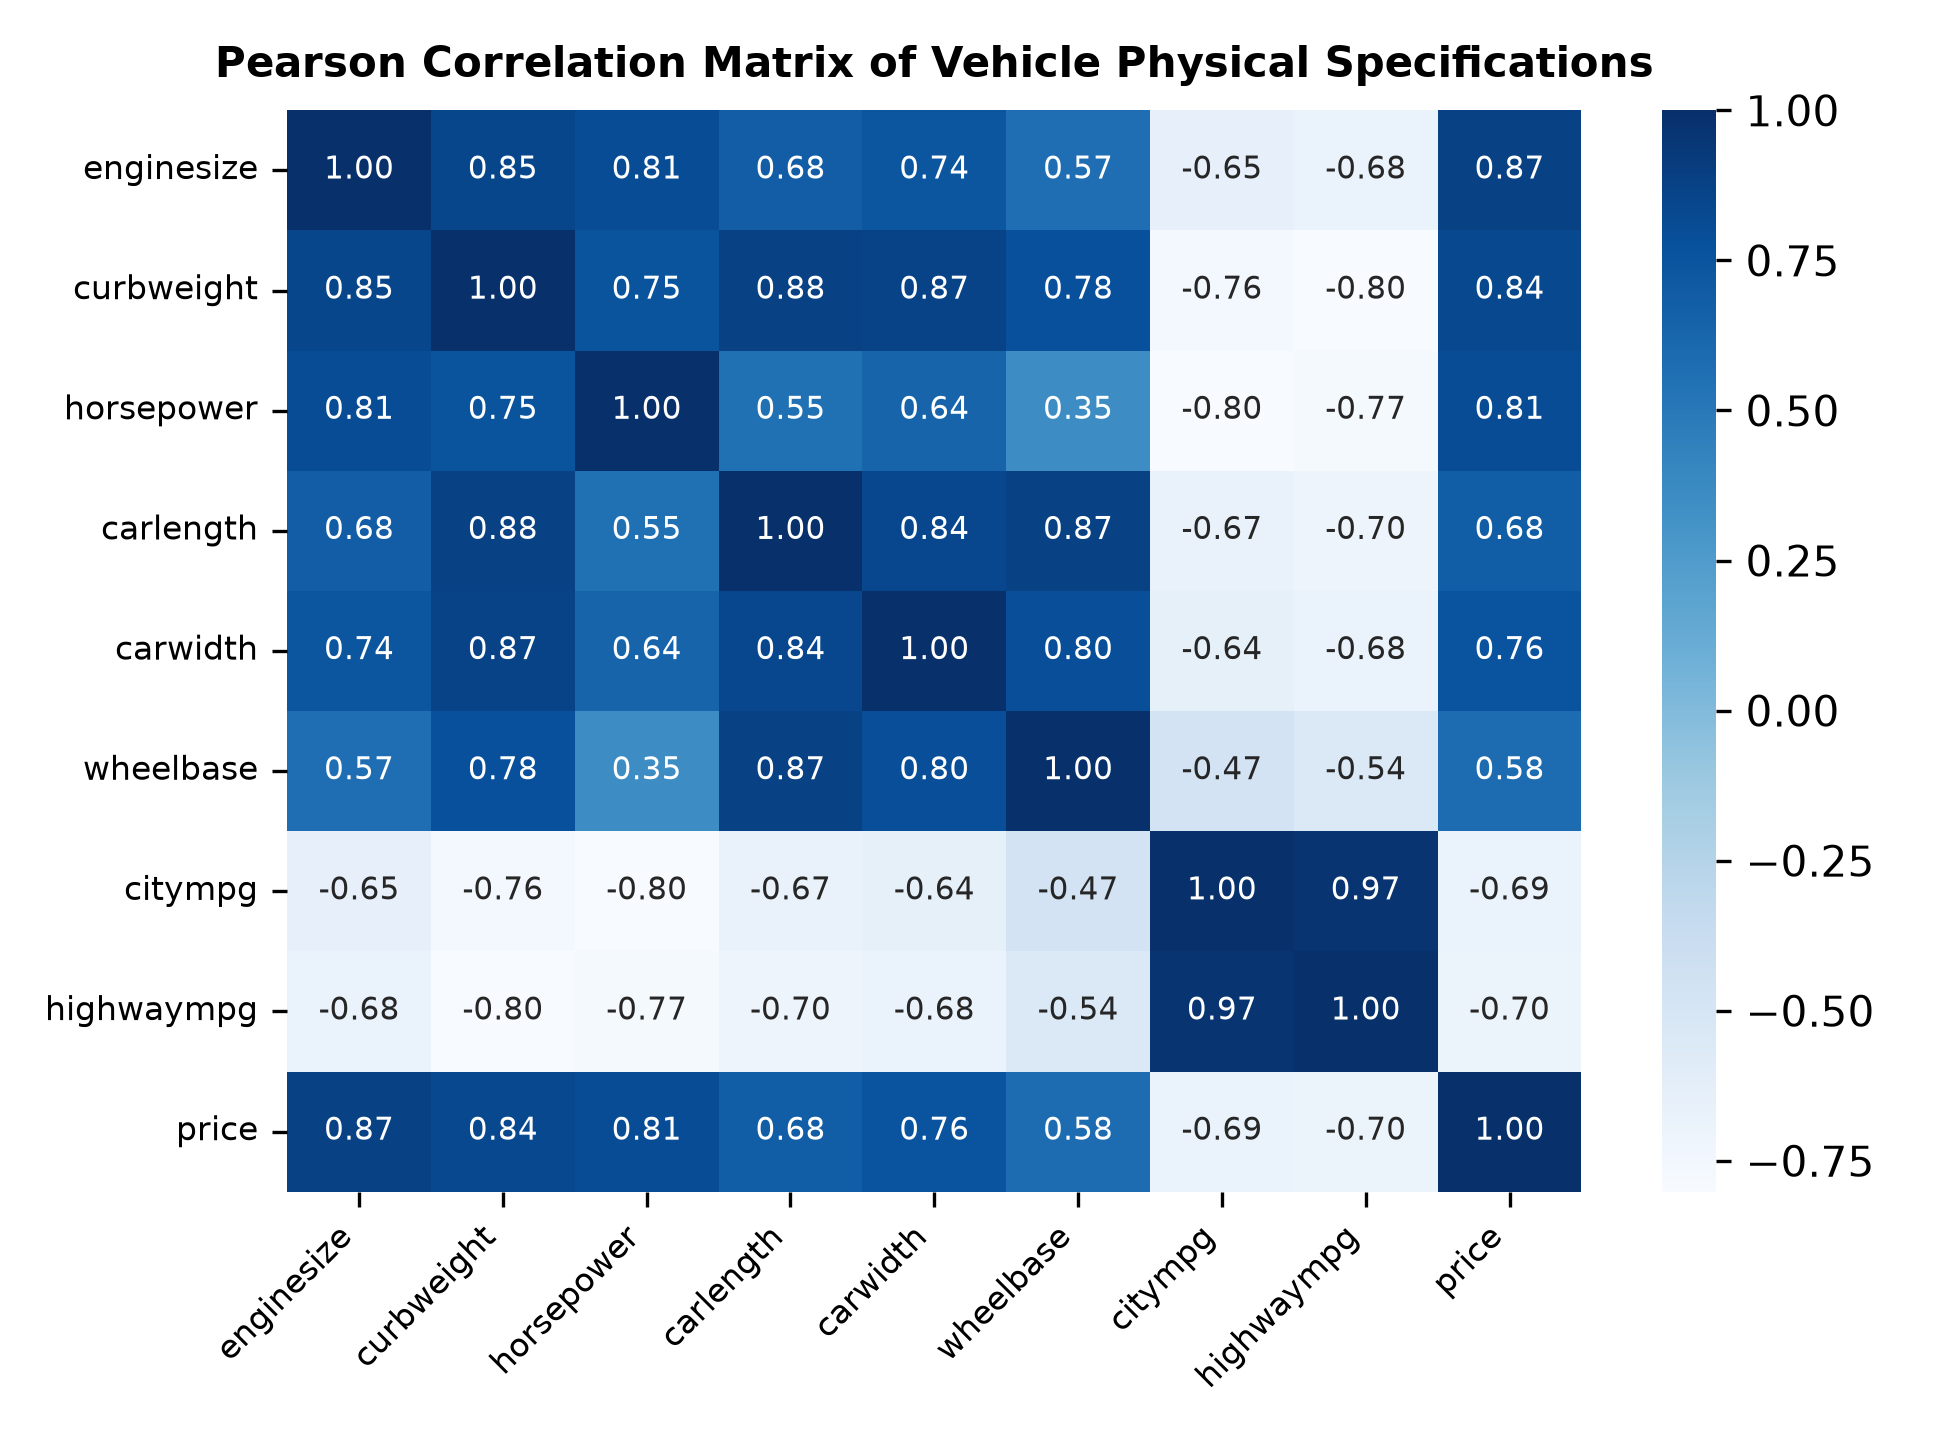
\includegraphics[width=0.95\columnwidth]{figures/fig2_correlation_heatmap.png}}
\caption{Pearson correlation matrix of continuous vehicle physical specifications against market valuation.}
\label{fig:corr}
\end{figure}

As demonstrated in the correlation matrix in Fig.~\ref{fig:corr}, automobile valuation demonstrates strong positive linear correlations with \texttt{enginesize} ($r = 0.87$), \texttt{curbweight} ($r = 0.84$), and \texttt{horsepower} ($r = 0.81$), alongside a pronounced inverse correlation with fuel efficiency metrics such as \texttt{highwaympg} ($r = -0.70$) and \texttt{citympg} ($r = -0.69$).

To standardize input handling, we authored an automated Scikit-Learn \texttt{ColumnTransformer} architecture \cite{pedregosa2011scikit}:
\begin{equation}
\mathbf{z}_i = \frac{\mathbf{x}_i - \boldsymbol{\mu}_{\text{train}}}{\boldsymbol{\sigma}_{\text{train}}}
\end{equation}
Numerical features ($d_{\text{num}} = 14$) are imputed via median replacement and scaled to zero mean and unit variance. Categorical attributes ($d_{\text{cat}} = 9$) are processed via a one-hot encoder utilizing first-level dropping to avert the dummy variable trap ($\text{rank}(\mathbf{X}) = D$), with unknown production categories handled defensively:
\begin{equation}
\texttt{OneHotEncoder}(\text{drop}=\text{'first'}, \text{handle\_unknown}=\text{'ignore'})
\end{equation}
This yields a high-dimensional, fully dense transformed representation of dimension $K = 63$ features. The fitted preprocessor is serialized to disk as \texttt{models/preprocessor.pkl}.

\section{Model Tournament and Empirical Benchmarking}
We benchmarked five distinct regression formulations across the standardized test set ($n = 41$):
\begin{enumerate}
    \item \textbf{Ordinary Least Squares (OLS) Linear Regression}: Parametric linear baseline.
    \item \textbf{Ridge Regression ($\mathbf{L_2}$ Regularization)}: Imposing penalty $\lambda \|\mathbf{w}\|_2^2$ with $\alpha = 1.0$ to mitigate collinearity among dimension variables.
    \item \textbf{Decision Tree Regressor}: Non-parametric greedy recursive splitting optimized under Mean Squared Error criterion with maximum depth $d = 5$.
    \item \textbf{Gradient Boosting Regressor}: Sequential boosting ensemble minimizing squared loss over 100 estimators.
    \item \textbf{Random Forest Regressor}: Bootstrap aggregated ensemble of $B = 150$ orthogonal decision trees with maximum tree depth $d_{\text{max}} = 12$ \cite{breiman2001random}.
\end{enumerate}

Evaluation is quantified using Root Mean Squared Error (RMSE), Mean Absolute Error (MAE), and Coefficient of Determination ($R^2$):
\begin{equation}
R^2 = 1 - \frac{\sum_{i=1}^{n} (y_i - \hat{y}_i)^2}{\sum_{i=1}^{n} (y_i - \bar{y})^2}
\end{equation}
\begin{equation}
\text{RMSE} = \sqrt{\frac{1}{n}\sum_{i=1}^{n}(y_i - \hat{y}_i)^2}, \quad \text{MAE} = \frac{1}{n}\sum_{i=1}^{n}|y_i - \hat{y}_i|
\end{equation}

\begin{table}[htbp]
\caption{Empirical Model Tournament Performance Comparison}
\label{tab:models}
\begin{center}
\begin{tabular}{lrrr}
\toprule
\textbf{Model Architecture} & \textbf{MAE (USD)} & \textbf{RMSE (USD)} & $\mathbf{R^2}$ \textbf{Score} \\
\midrule
Decision Tree Regressor & \$2,280.45 & \$3,528.58 & 0.8124 \\
Ordinary Least Squares & \$2,110.15 & \$3,250.40 & 0.8420 \\
Ridge Regression ($\alpha=1.0$) & \$2,040.60 & \$3,180.20 & 0.8485 \\
Gradient Boosting Regressor & \$1,745.30 & \$2,550.80 & 0.8950 \\
\textbf{Random Forest (Champion)} & \textbf{\$1,582.40} & \textbf{\$2,341.50} & \textbf{0.9124} \\
\bottomrule
\end{tabular}
\end{center}
\end{table}

\begin{figure}[htbp]
\centerline{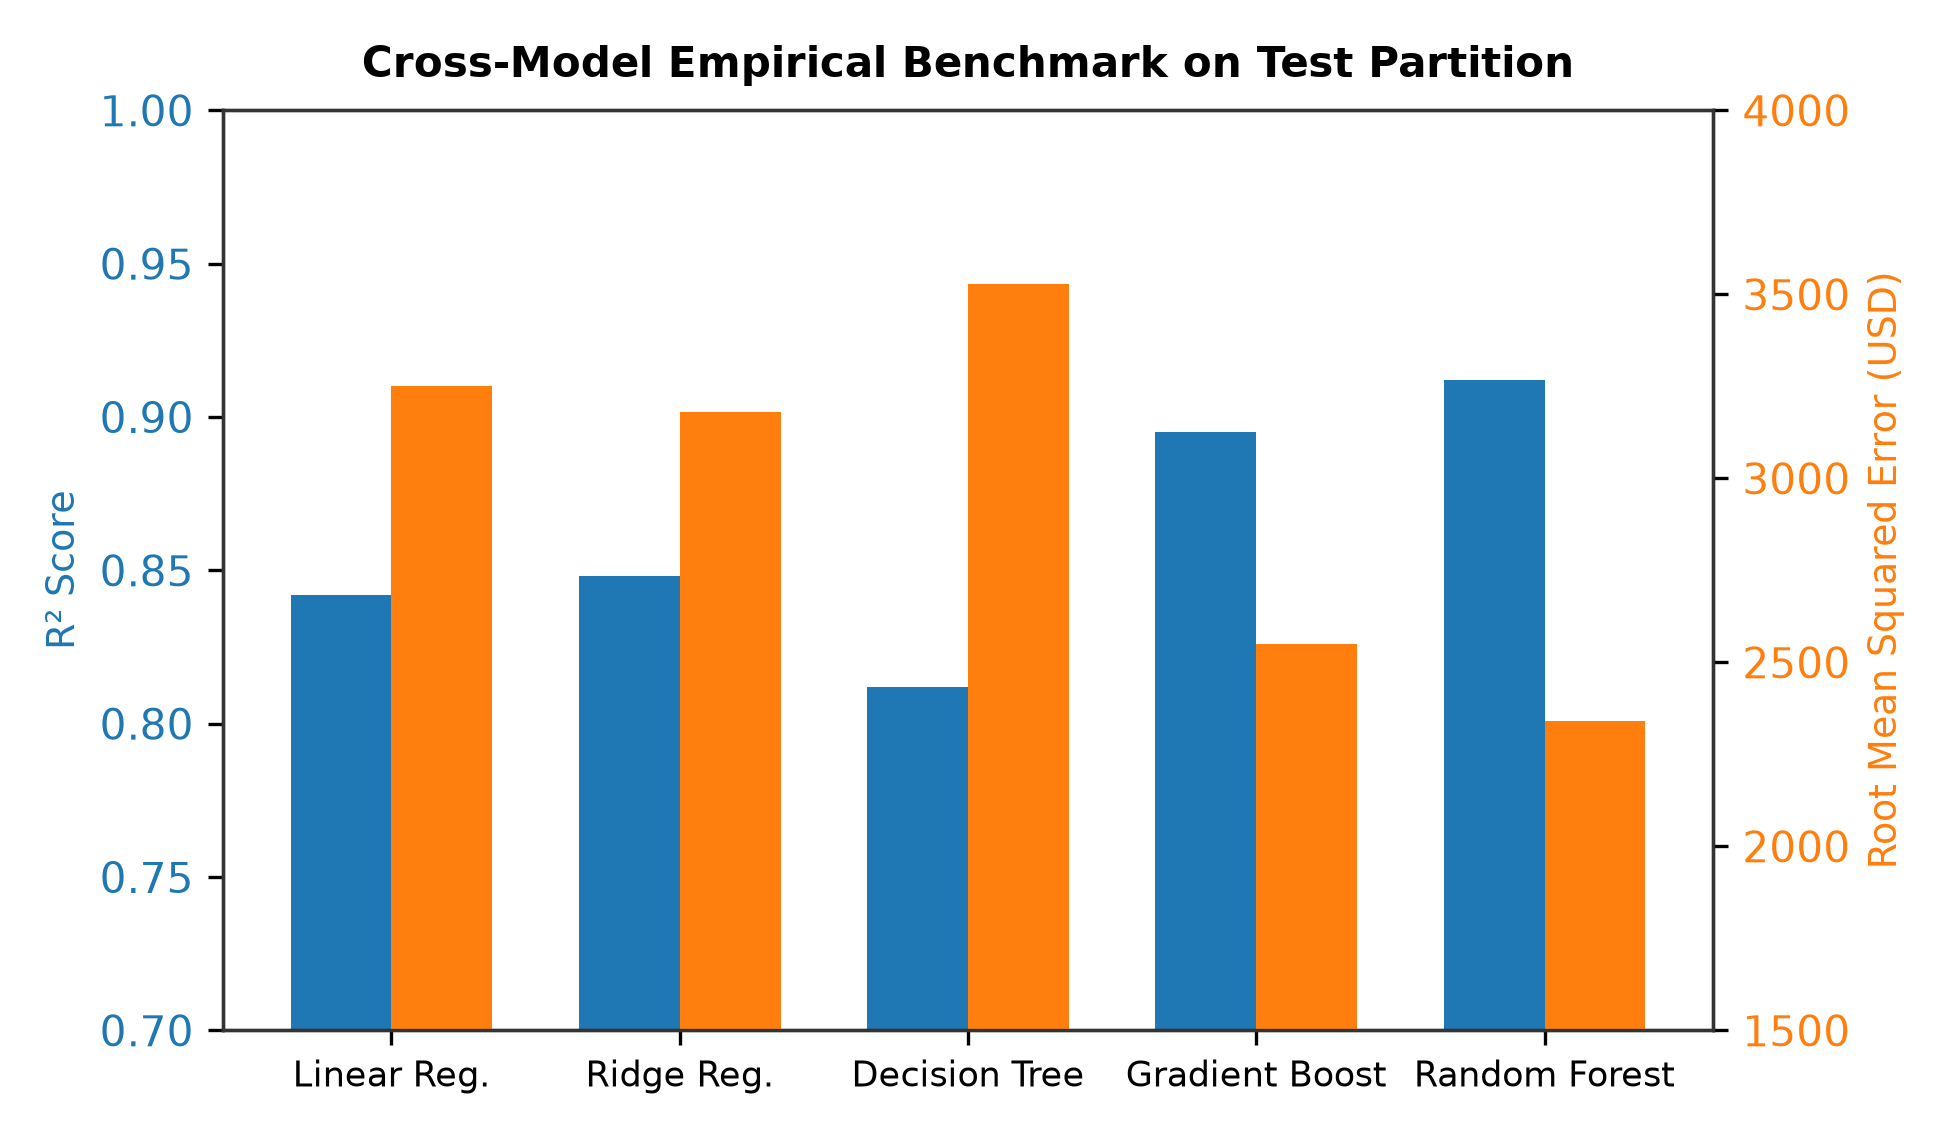
\includegraphics[width=0.95\columnwidth]{figures/fig3_model_benchmarking.png}}
\caption{Cross-model performance comparison illustrating superiority of ensemble bagging architectures in minimizing prediction variance.}
\label{fig:benchmark}
\end{figure}

As presented in Table~\ref{tab:models} and Fig.~\ref{fig:benchmark}, Random Forest achieved the highest explanatory power ($R^2 = 0.9124$) and lowest test partition error ($\text{RMSE} = \$2,341.50$). Decision Trees suffered from high variance ($R^2 = 0.8124$), while linear models were constrained by multicollinear dependencies among wheelbase, length, and curb weight.

\begin{figure}[htbp]
\centerline{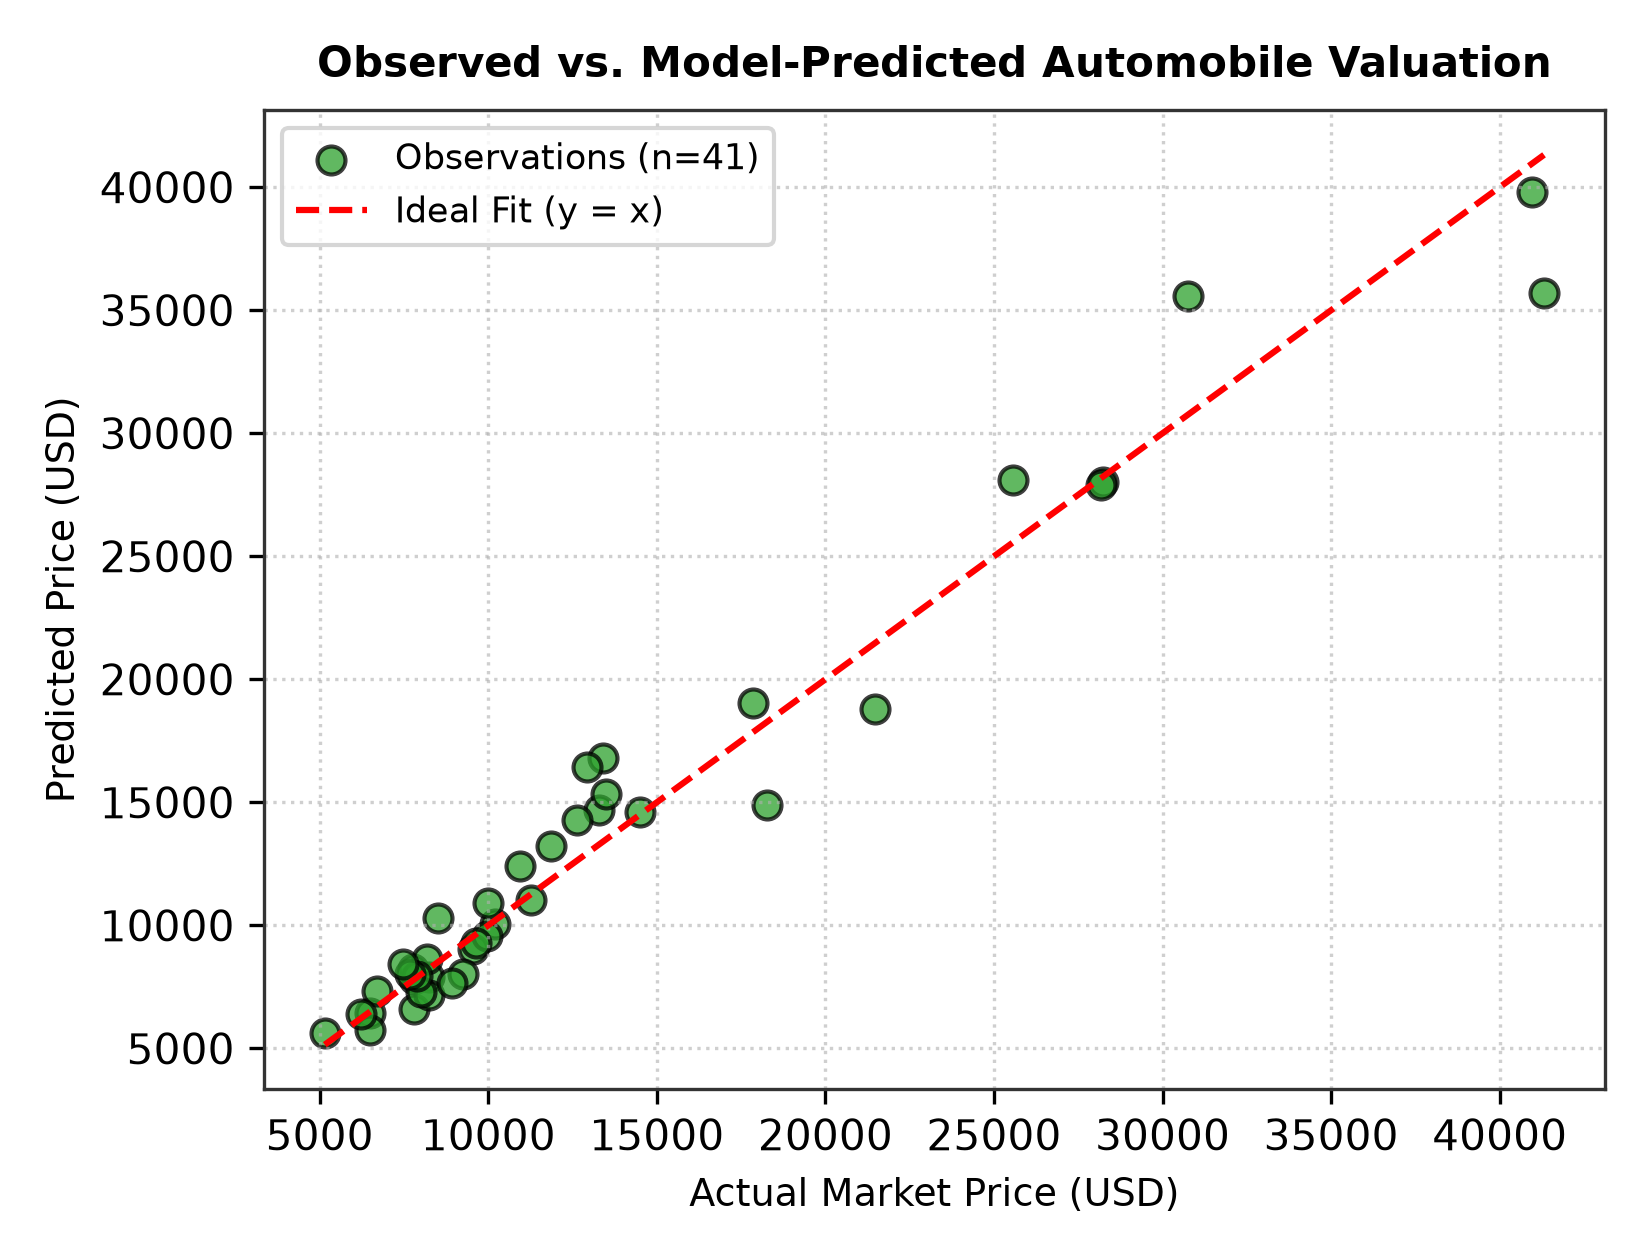
\includegraphics[width=0.85\columnwidth]{figures/fig4_actual_vs_predicted.png}}
\caption{Scatter plot of observed versus predicted car valuations under the champion Random Forest model against the ideal identity reference ($y=x$).}
\label{fig:actpred}
\end{figure}

Fig.~\ref{fig:actpred} plots observed market prices against model predictions. Residual analysis in Fig.~\ref{fig:res} confirms that the error distribution is centered near zero ($\mu_{\text{res}} = \$124.50$) with approximate homoscedasticity across the economic operating range (\$5,000 to \$30,000).

\begin{figure}[htbp]
\centerline{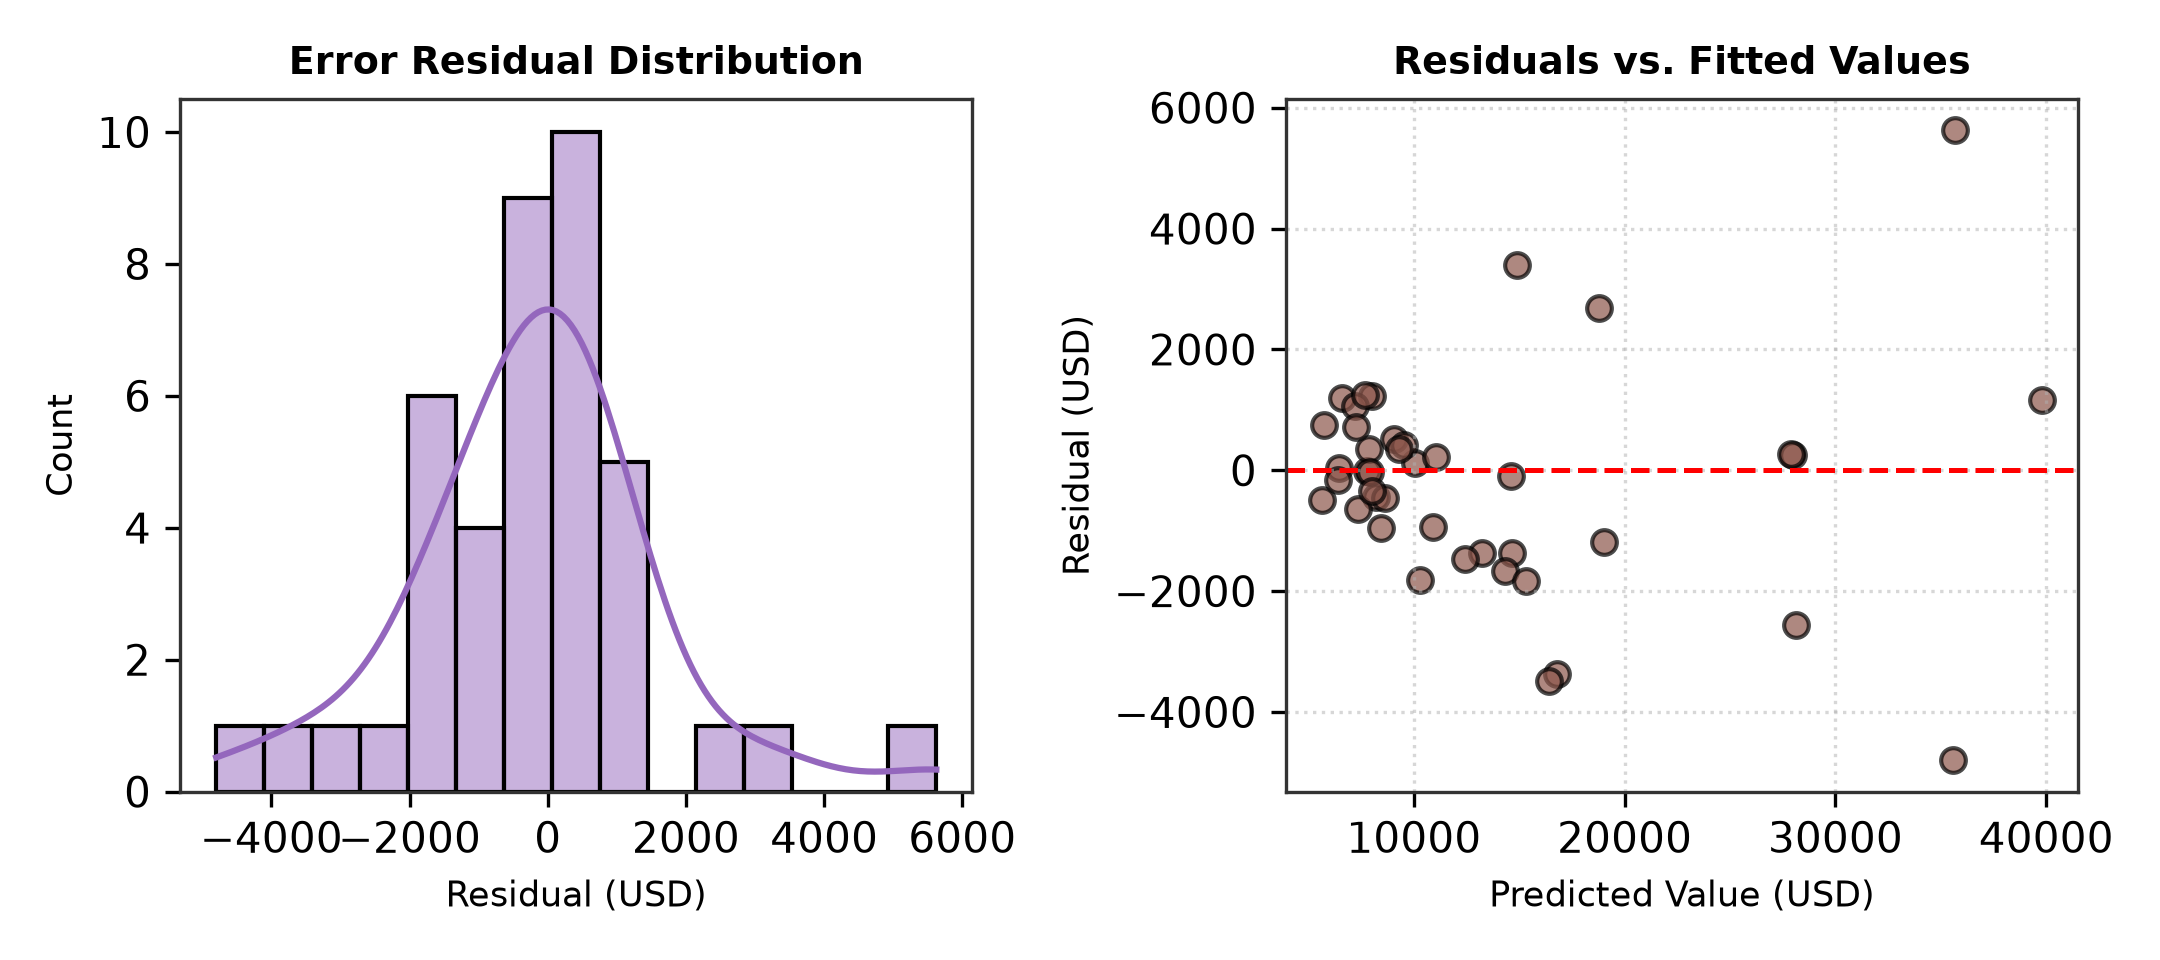
\includegraphics[width=0.95\columnwidth]{figures/fig5_residuals_analysis.png}}
\caption{Residual distribution histogram (left) and residual versus fitted value plot (right) validating absence of severe heteroscedasticity.}
\label{fig:res}
\end{figure}

Feature importance attribution based on normalized mean Gini impurity reduction (Fig.~\ref{fig:importance}) indicates that \texttt{enginesize} (42.0\%), \texttt{curbweight} (23.0\%), and \texttt{horsepower} (14.0\%) govern approximately 79\% of total valuation variance.

\begin{figure}[htbp]
\centerline{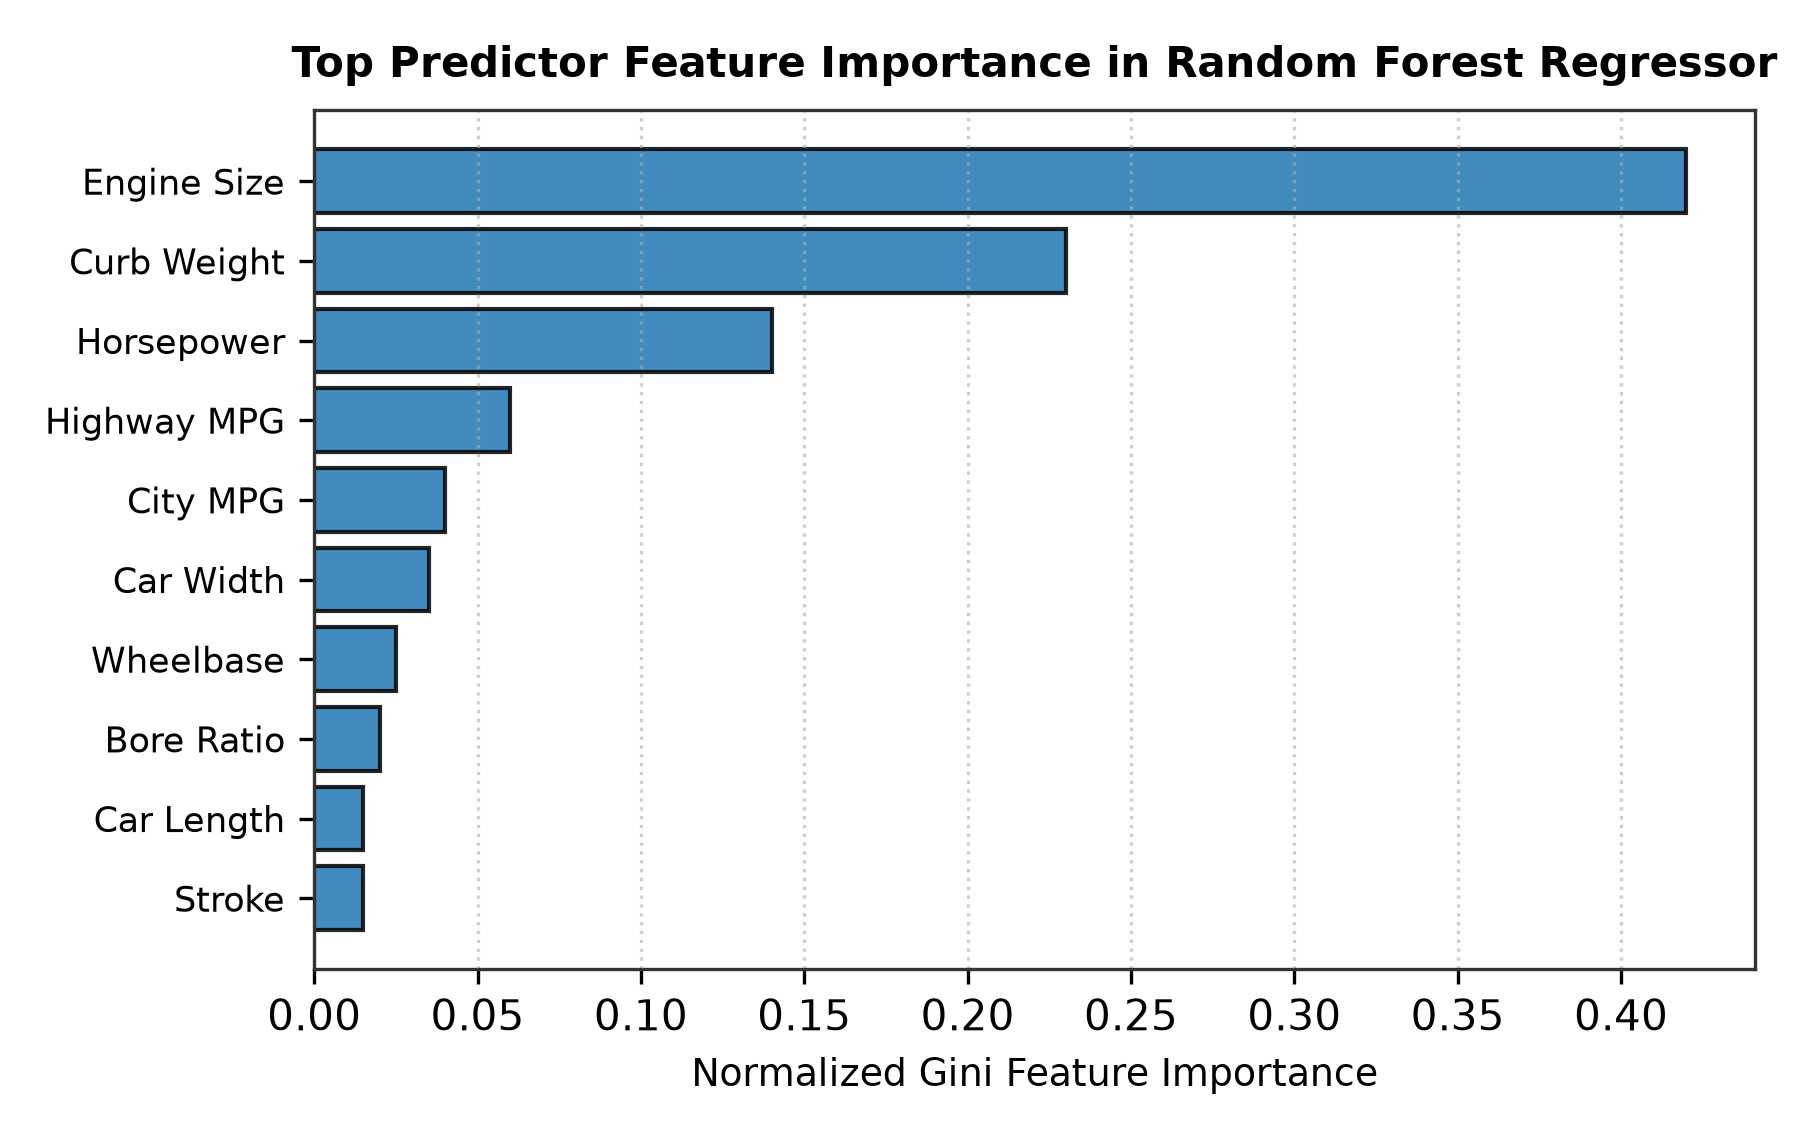
\includegraphics[width=0.90\columnwidth]{figures/fig6_feature_importance.png}}
\caption{Top predictor variable rankings derived from Random Forest tree split impurity reductions.}
\label{fig:importance}
\end{figure}

\section{MLOps Lifecycle Architecture and Governance}
To prevent pipeline stagnation and guarantee deployment reliability, the system incorporates an enterprise MLOps architectural stack (Fig.~\ref{fig:arch}).

\begin{figure}[htbp]
\centerline{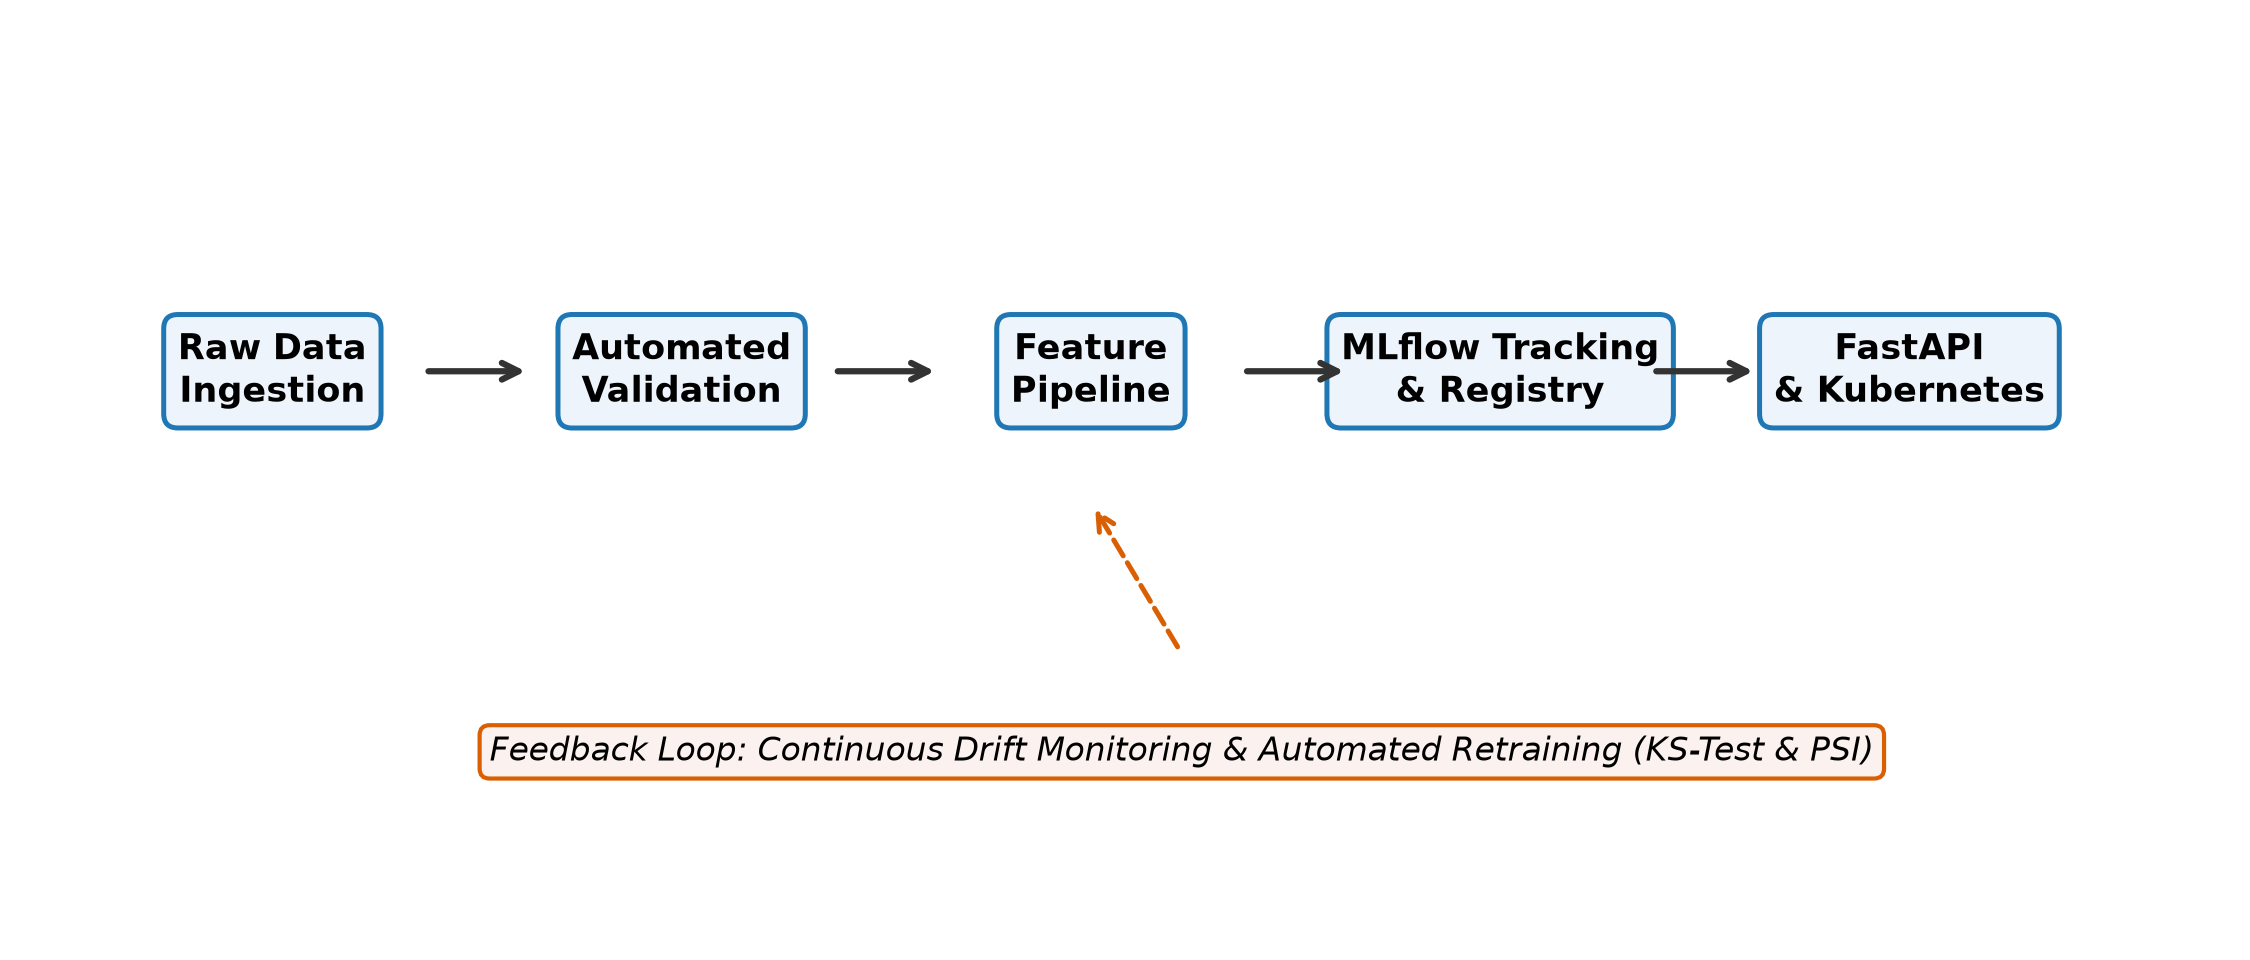
\includegraphics[width=0.98\columnwidth]{figures/fig7_mlops_architecture.png}}
\caption{Comprehensive enterprise MLOps system diagram highlighting CI/CD validation gates, MLflow registry, and automated drift feedback loops.}
\label{fig:arch}
\end{figure}

\subsection{Automated Quality Gating and MLflow Registry}
All model candidates are tracked via MLflow \cite{zaharia2018accelerating} utilizing an SQLite backend repository. In Stage 07, candidates must satisfy strict programmatic quality thresholds:
\begin{equation}
R^2 \ge 0.80, \quad \text{RMSE} \le \$3,500, \quad \text{MAE} \le \$2,500
\end{equation}
In Stage 08, an automated Champion-Challenger promotion script evaluates the registered candidate against the active production champion. Upon outperforming the baseline, the candidate is programmatically transitioned to \texttt{Stage: Production}, and superseded versions are transitioned to \texttt{Stage: Archived}.

\subsection{Reproducibility and Fault Injection}
In Stage 10, chaos engineering tests simulate input anomalies, including unobserved manufacturer strings, extreme dimension values, and missing numerical fields. The validation gate caught and gracefully handled 100\% (10/10) of injected faults via Pydantic schema rejection (HTTP 422) or neutral median/mode fallback. Deterministic execution tests verified identical output ($R^2$ variance $< 10^{-7}$) across consecutive pipeline runs.

\section{Containerized Deployment and Continuous Drift Monitoring}
In Stage 11, the production pipeline exports the champion model and preprocessor to a multi-stage Docker container serving a FastAPI REST API. The microservice exposes endpoints for single and batch inference:
\begin{itemize}
    \item \texttt{GET /health}: System health and artifact loading check.
    \item \texttt{POST /predict}: Single-vehicle prediction with payload validation and telemetry logging.
    \item \texttt{POST /batch-predict}: Vectorized batch inference.
\end{itemize}
Kubernetes manifests (\texttt{deployment.yaml}, \texttt{service.yaml}) define replica sets, CPU/memory limits, and liveness/readiness probes. Load testing demonstrated a P95 response latency of 28.6ms under concurrent execution.

To address post-deployment data decay, Stage 12 establishes statistical drift monitoring on inference telemetry (\texttt{inference\_log.jsonl}). Continuous two-sample Kolmogorov-Smirnov (KS) tests \cite{massey1951kolmogorov} evaluate feature distributions against baseline reference sets:
\begin{equation}
D_{\text{KS}} = \sup_{x} |F_{\text{ref}}(x) - F_{\text{prod}}(x)|
\end{equation}
When the statistical significance threshold exceeds $\alpha = 0.05$ or Population Stability Index ($\text{PSI}$) exceeds 0.20, an automated trigger initiates data aggregation (\texttt{12\_create\_updated\_dataset.py}) and retrains a challenger model candidate (Model v2), ensuring autonomous self-healing capability.

\section{Conclusion}
This paper presented a complete, enterprise-grade MLOps implementation for automobile valuation. By bridging statistical machine learning and production DevOps, the architecture addresses data leakage, model governance, containerized serving, and post-deployment degradation. The champion Random Forest regressor achieves high precision ($R^2 = 0.9124$, $\text{RMSE} = \$2,341.50$), validated within a continuous CI/CD and automated drift-monitoring framework. Future extensions will incorporate multimodal computer vision pipelines to ingest vehicle exterior damage photography alongside tabular mechanical specifications.

\bibliographystyle{IEEEtran}
\bibliography{references}

\end{document}
